\documentclass[]{article}
\usepackage{lmodern}
\usepackage{amssymb,amsmath}
\usepackage{ifxetex,ifluatex}
\usepackage{fixltx2e} % provides \textsubscript
\ifnum 0\ifxetex 1\fi\ifluatex 1\fi=0 % if pdftex
  \usepackage[T1]{fontenc}
  \usepackage[utf8]{inputenc}
\else % if luatex or xelatex
  \ifxetex
    \usepackage{mathspec}
  \else
    \usepackage{fontspec}
  \fi
  \defaultfontfeatures{Ligatures=TeX,Scale=MatchLowercase}
\fi
% use upquote if available, for straight quotes in verbatim environments
\IfFileExists{upquote.sty}{\usepackage{upquote}}{}
% use microtype if available
\IfFileExists{microtype.sty}{%
\usepackage{microtype}
\UseMicrotypeSet[protrusion]{basicmath} % disable protrusion for tt fonts
}{}
\usepackage[margin=1in]{geometry}
\usepackage{hyperref}
\hypersetup{unicode=true,
            pdftitle={Trabalho de dados Binários},
            pdfauthor={Laís Hoffmann, Simone Matsubara, Yasmin Fernandes, Willian Meira},
            pdfborder={0 0 0},
            breaklinks=true}
\urlstyle{same}  % don't use monospace font for urls
\usepackage{color}
\usepackage{fancyvrb}
\newcommand{\VerbBar}{|}
\newcommand{\VERB}{\Verb[commandchars=\\\{\}]}
\DefineVerbatimEnvironment{Highlighting}{Verbatim}{commandchars=\\\{\}}
% Add ',fontsize=\small' for more characters per line
\usepackage{framed}
\definecolor{shadecolor}{RGB}{248,248,248}
\newenvironment{Shaded}{\begin{snugshade}}{\end{snugshade}}
\newcommand{\KeywordTok}[1]{\textcolor[rgb]{0.13,0.29,0.53}{\textbf{#1}}}
\newcommand{\DataTypeTok}[1]{\textcolor[rgb]{0.13,0.29,0.53}{#1}}
\newcommand{\DecValTok}[1]{\textcolor[rgb]{0.00,0.00,0.81}{#1}}
\newcommand{\BaseNTok}[1]{\textcolor[rgb]{0.00,0.00,0.81}{#1}}
\newcommand{\FloatTok}[1]{\textcolor[rgb]{0.00,0.00,0.81}{#1}}
\newcommand{\ConstantTok}[1]{\textcolor[rgb]{0.00,0.00,0.00}{#1}}
\newcommand{\CharTok}[1]{\textcolor[rgb]{0.31,0.60,0.02}{#1}}
\newcommand{\SpecialCharTok}[1]{\textcolor[rgb]{0.00,0.00,0.00}{#1}}
\newcommand{\StringTok}[1]{\textcolor[rgb]{0.31,0.60,0.02}{#1}}
\newcommand{\VerbatimStringTok}[1]{\textcolor[rgb]{0.31,0.60,0.02}{#1}}
\newcommand{\SpecialStringTok}[1]{\textcolor[rgb]{0.31,0.60,0.02}{#1}}
\newcommand{\ImportTok}[1]{#1}
\newcommand{\CommentTok}[1]{\textcolor[rgb]{0.56,0.35,0.01}{\textit{#1}}}
\newcommand{\DocumentationTok}[1]{\textcolor[rgb]{0.56,0.35,0.01}{\textbf{\textit{#1}}}}
\newcommand{\AnnotationTok}[1]{\textcolor[rgb]{0.56,0.35,0.01}{\textbf{\textit{#1}}}}
\newcommand{\CommentVarTok}[1]{\textcolor[rgb]{0.56,0.35,0.01}{\textbf{\textit{#1}}}}
\newcommand{\OtherTok}[1]{\textcolor[rgb]{0.56,0.35,0.01}{#1}}
\newcommand{\FunctionTok}[1]{\textcolor[rgb]{0.00,0.00,0.00}{#1}}
\newcommand{\VariableTok}[1]{\textcolor[rgb]{0.00,0.00,0.00}{#1}}
\newcommand{\ControlFlowTok}[1]{\textcolor[rgb]{0.13,0.29,0.53}{\textbf{#1}}}
\newcommand{\OperatorTok}[1]{\textcolor[rgb]{0.81,0.36,0.00}{\textbf{#1}}}
\newcommand{\BuiltInTok}[1]{#1}
\newcommand{\ExtensionTok}[1]{#1}
\newcommand{\PreprocessorTok}[1]{\textcolor[rgb]{0.56,0.35,0.01}{\textit{#1}}}
\newcommand{\AttributeTok}[1]{\textcolor[rgb]{0.77,0.63,0.00}{#1}}
\newcommand{\RegionMarkerTok}[1]{#1}
\newcommand{\InformationTok}[1]{\textcolor[rgb]{0.56,0.35,0.01}{\textbf{\textit{#1}}}}
\newcommand{\WarningTok}[1]{\textcolor[rgb]{0.56,0.35,0.01}{\textbf{\textit{#1}}}}
\newcommand{\AlertTok}[1]{\textcolor[rgb]{0.94,0.16,0.16}{#1}}
\newcommand{\ErrorTok}[1]{\textcolor[rgb]{0.64,0.00,0.00}{\textbf{#1}}}
\newcommand{\NormalTok}[1]{#1}
\usepackage{graphicx,grffile}
\makeatletter
\def\maxwidth{\ifdim\Gin@nat@width>\linewidth\linewidth\else\Gin@nat@width\fi}
\def\maxheight{\ifdim\Gin@nat@height>\textheight\textheight\else\Gin@nat@height\fi}
\makeatother
% Scale images if necessary, so that they will not overflow the page
% margins by default, and it is still possible to overwrite the defaults
% using explicit options in \includegraphics[width, height, ...]{}
\setkeys{Gin}{width=\maxwidth,height=\maxheight,keepaspectratio}
\IfFileExists{parskip.sty}{%
\usepackage{parskip}
}{% else
\setlength{\parindent}{0pt}
\setlength{\parskip}{6pt plus 2pt minus 1pt}
}
\setlength{\emergencystretch}{3em}  % prevent overfull lines
\providecommand{\tightlist}{%
  \setlength{\itemsep}{0pt}\setlength{\parskip}{0pt}}
\setcounter{secnumdepth}{0}
% Redefines (sub)paragraphs to behave more like sections
\ifx\paragraph\undefined\else
\let\oldparagraph\paragraph
\renewcommand{\paragraph}[1]{\oldparagraph{#1}\mbox{}}
\fi
\ifx\subparagraph\undefined\else
\let\oldsubparagraph\subparagraph
\renewcommand{\subparagraph}[1]{\oldsubparagraph{#1}\mbox{}}
\fi

%%% Use protect on footnotes to avoid problems with footnotes in titles
\let\rmarkdownfootnote\footnote%
\def\footnote{\protect\rmarkdownfootnote}

%%% Change title format to be more compact
\usepackage{titling}

% Create subtitle command for use in maketitle
\newcommand{\subtitle}[1]{
  \posttitle{
    \begin{center}\large#1\end{center}
    }
}

\setlength{\droptitle}{-2em}
  \title{Trabalho de dados Binários}
  \pretitle{\vspace{\droptitle}\centering\huge}
  \posttitle{\par}
\subtitle{Acidentes de carro}
  \author{Laís Hoffmann, Simone Matsubara, Yasmin Fernandes, Willian Meira}
  \preauthor{\centering\large\emph}
  \postauthor{\par}
  \predate{\centering\large\emph}
  \postdate{\par}
  \date{2018-11-13}

\usepackage[brazil]{babel} \usepackage{amsmath} \usepackage{float}
\usepackage{bm}

\begin{document}
\maketitle

\hypertarget{base-de-dados}{%
\section{1. Base de Dados}\label{base-de-dados}}

\textbf{1.1 Descrição dos dados}

Os dados foram retirados do pacote ``DAAG'', sendo dados dos EUA, entre
1997-2002, de acidentes de carro relatados pela polícia nos quais há um
evento prejudicial (pessoas ou propriedade) e do qual pelo menos um
veículo foi rebocado. Os dados são restritos aos ocupantes do banco da
frente, incluem apenas um subconjunto das variáveis registradas e são
restritos de outras maneiras também.

A base original possui uma base de dados com 26.217 observações nas 15
variáveis a seguir.

1 - \textbf{veloc}: velocidades estimadas do impacto do acidente:
1-9km/h, 10-24, 25-39, 40-54, 55+ \newline 2 - \textbf{pesos}: Pesos de
observação \newline 3 - \textbf{sobrev}: Classificação se sobreviveu ao
acidente: 1 = morreu ou 0 = sobreviveu \newline 4 - \textbf{airbag}: Se
o carro possui airbag: com ou sem airbag \newline 5 - \textbf{cinto}:
uso do cinto de segurança: com ou sem cinto \newline 6 -
\textbf{frontal}: impacto do acidente: 0 = não frontal, 1 = impacto
frontal \newline 7 - \textbf{sexo}: Sexo: 0 = Feminino ou 1 = Masculino
\newline 8 - \textbf{idade}: Idade dos ocupantes do veículo \newline 9 -
\textbf{anoaci}: Ano do acidente (1997-2002) \newline 10 -
\textbf{anovei}: Ano do veículo (1953-2003) \newline 11 -
\textbf{airbagcat}: Se Airbags foram acionados: deploy, nodeploy,
unavail \newline 12 - \textbf{ocupantes}: Posição do airbag acionado:
driver, pass \newline 13 - \textbf{abfunc}: Airbag acionados: 0: Se não
possuia airbag ou não foi acionado, 1: Um ou mais airbags foram
acionados \newline 14 - \textbf{grav}: Gravidade do acidente: 0:none, 1
= Possível Lesão, 2:no incapacity, 3:incapacity, 4:killed; 5:unknown,
6:prior death \newline 15 - \textbf{numcaso}: Número do caso.

No entanto, escolhemos analisar os dados do ano do acidente de 2002 e
veículos de ano 2000 e retirar as variaveis weight, abcat e caseid.

\hypertarget{analise-descritiva}{%
\section{2 Análise Descritiva}\label{analise-descritiva}}

\textbf{2.1 Medidas de Resumo}

\begin{Shaded}
\begin{Highlighting}[]
\KeywordTok{summary}\NormalTok{(dados[ , }\KeywordTok{c}\NormalTok{(}\DecValTok{1}\OperatorTok{:}\DecValTok{8}\NormalTok{,}\DecValTok{10}\NormalTok{)])}
\end{Highlighting}
\end{Shaded}

\begin{verbatim}
##    veloc       sobrev      airbag      cinto       frontal    
##  01-09:  686   Nao: 1180   Nao:11798   Nao: 7644   Nao: 9351  
##  10-24:12848   Sim:25037   Sim:14419   Sim:18573   Sim:16866  
##  25-39: 8214                                                  
##  40-54: 2977                                                  
##  55+  : 1492                                                  
##                                                               
##                                                               
##    sexo           idade            ocupantes          grav     
##  Fem :12248   Min.   :16.00   Motorista :20601   3      :8495  
##  Masc:13969   1st Qu.:22.00   Passageiro: 5616   0      :6479  
##               Median :33.00                      1      :5595  
##               Mean   :37.21                      2      :4242  
##               3rd Qu.:48.00                      4      :1118  
##               Max.   :97.00                      (Other): 135  
##                                                  NA's   : 153
\end{verbatim}

\#\#\#Nota-se na varável velocidade uma frequência maior na faixa 10-24
milhas. \#\#\#A maioria estava com cinto de segurança e os acidentes
foram a maioria frontais. \textbf{2.3 Histogramas}

\begin{Shaded}
\begin{Highlighting}[]
\KeywordTok{par}\NormalTok{(}\DataTypeTok{mfrow =} \KeywordTok{c}\NormalTok{(}\DecValTok{3}\NormalTok{,}\DecValTok{3}\NormalTok{))}
\KeywordTok{plot}\NormalTok{(dados}\OperatorTok{$}\NormalTok{abfunc, }\DataTypeTok{xlab =} \StringTok{''}\NormalTok{, }\DataTypeTok{ylab =} \StringTok{''}\NormalTok{, }\DataTypeTok{main =} \StringTok{'AB Funcionou'}\NormalTok{)}
\KeywordTok{plot}\NormalTok{(dados}\OperatorTok{$}\NormalTok{veloc, }\DataTypeTok{xlab =} \StringTok{''}\NormalTok{, }\DataTypeTok{ylab =} \StringTok{''}\NormalTok{, }\DataTypeTok{main =} \StringTok{'Velocidade'}\NormalTok{)}
\KeywordTok{plot}\NormalTok{(dados}\OperatorTok{$}\NormalTok{sobrev, }\DataTypeTok{xlab =} \StringTok{''}\NormalTok{, }\DataTypeTok{ylab =} \StringTok{''}\NormalTok{, }\DataTypeTok{main =} \StringTok{'Sobrevivente'}\NormalTok{)}
\KeywordTok{plot}\NormalTok{(dados}\OperatorTok{$}\NormalTok{airbag, }\DataTypeTok{xlab =} \StringTok{''}\NormalTok{, }\DataTypeTok{ylab =} \StringTok{''}\NormalTok{, }\DataTypeTok{main =} \StringTok{'Airbag'}\NormalTok{)}
\KeywordTok{plot}\NormalTok{(dados}\OperatorTok{$}\NormalTok{cinto, }\DataTypeTok{xlab =} \StringTok{''}\NormalTok{, }\DataTypeTok{ylab =} \StringTok{''}\NormalTok{, }\DataTypeTok{main =} \StringTok{'Cinto'}\NormalTok{)}
\KeywordTok{plot}\NormalTok{(dados}\OperatorTok{$}\NormalTok{frontal, }\DataTypeTok{xlab =} \StringTok{''}\NormalTok{, }\DataTypeTok{ylab =} \StringTok{''}\NormalTok{, }\DataTypeTok{main =} \StringTok{'Frontal'}\NormalTok{)}
\KeywordTok{plot}\NormalTok{(dados}\OperatorTok{$}\NormalTok{sexo, }\DataTypeTok{xlab =} \StringTok{''}\NormalTok{, }\DataTypeTok{ylab =} \StringTok{''}\NormalTok{, }\DataTypeTok{main =} \StringTok{'Sexo'}\NormalTok{)}
\KeywordTok{plot}\NormalTok{(dados}\OperatorTok{$}\NormalTok{ocupantes, }\DataTypeTok{xlab =} \StringTok{''}\NormalTok{, }\DataTypeTok{ylab =} \StringTok{''}\NormalTok{, }\DataTypeTok{main =} \StringTok{'Ocupante'}\NormalTok{)}
\KeywordTok{plot}\NormalTok{(dados}\OperatorTok{$}\NormalTok{grav, }\DataTypeTok{xlab =} \StringTok{''}\NormalTok{, }\DataTypeTok{ylab =} \StringTok{''}\NormalTok{, }\DataTypeTok{main =} \StringTok{'Gravidade'}\NormalTok{)}
\KeywordTok{mtext}\NormalTok{(}\DataTypeTok{side=}\DecValTok{2}\NormalTok{,}\DataTypeTok{cex=}\FloatTok{1.3}\NormalTok{,}\DataTypeTok{line=}\OperatorTok{-}\FloatTok{1.5}\NormalTok{,}\DataTypeTok{text=}\StringTok{"Frequencias"}\NormalTok{,}\DataTypeTok{outer=}\OtherTok{TRUE}\NormalTok{)}
\end{Highlighting}
\end{Shaded}

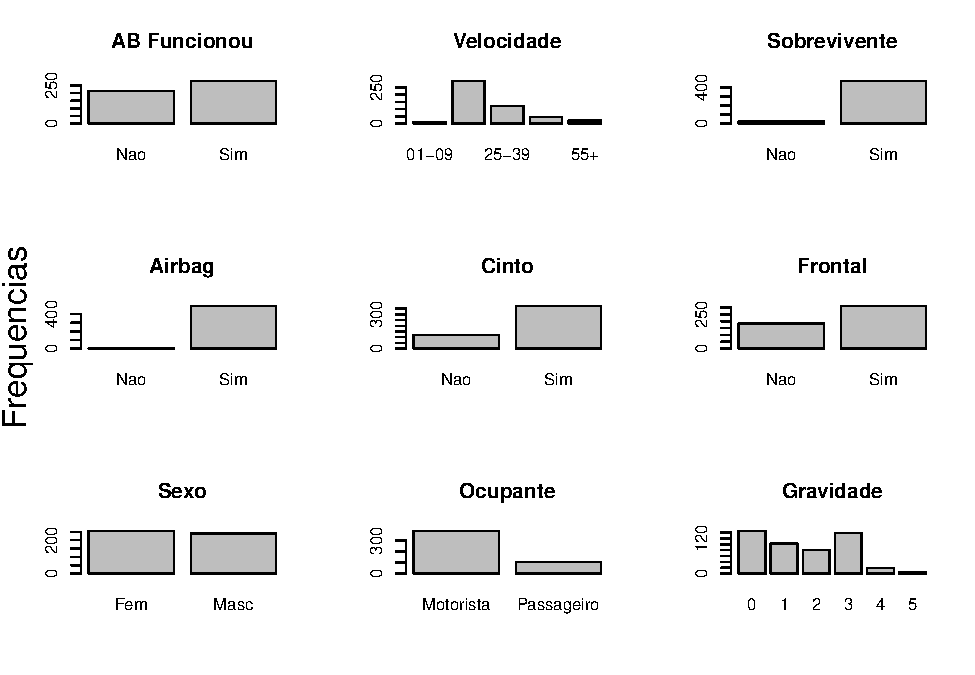
\includegraphics{Dados_Binários1_files/figure-latex/unnamed-chunk-5-1.pdf}

\textbf{2.4 Distribuição}

\begin{Shaded}
\begin{Highlighting}[]
\NormalTok{g1<-}\KeywordTok{ggplot}\NormalTok{(dados, }\KeywordTok{aes}\NormalTok{(}\DataTypeTok{y=}\NormalTok{idade)) }\OperatorTok{+}\StringTok{ }
\StringTok{  }\KeywordTok{geom_boxplot}\NormalTok{()}\OperatorTok{+}\StringTok{ }\KeywordTok{xlab}\NormalTok{(}\StringTok{'idade'}\NormalTok{)}\OperatorTok{+}\StringTok{ }\KeywordTok{ylab}\NormalTok{(}\StringTok{''}\NormalTok{) }\OperatorTok{+}
\StringTok{  }\KeywordTok{theme}\NormalTok{(}\DataTypeTok{legend.title=}\KeywordTok{element_blank}\NormalTok{())}


\NormalTok{g1}
\end{Highlighting}
\end{Shaded}

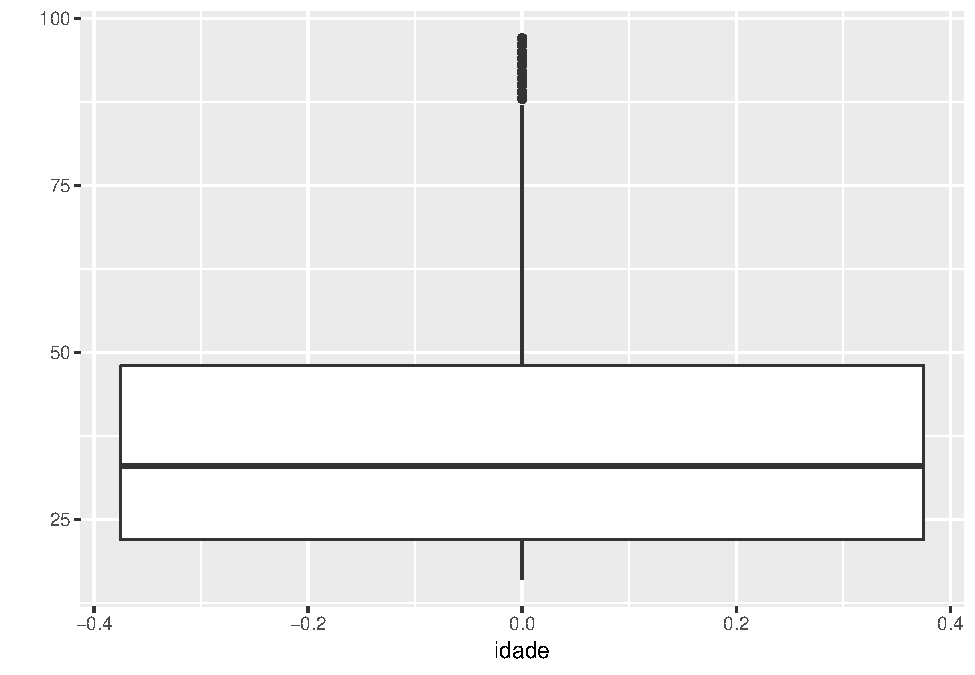
\includegraphics{Dados_Binários1_files/figure-latex/unnamed-chunk-6-1.pdf}
\#\#\#Intuitivamente sabemos que para nosso escopo a variável idade não
é significativa para o nosso modelo porém para comprovar adiante faremos
um teste para evidênciar a irrelevancia da variável no modelo.

\hypertarget{ajuste-do-modelo-de-regressao}{%
\section{3. Ajuste do Modelo de
Regressão}\label{ajuste-do-modelo-de-regressao}}

\#\#\textbf{3.1 Ligação Logito}

Vamos ajustar um Modelo Linear Generalizado Binomial com função de
ligação Logito. A expressão do modelo é dada por:

\(ln (\frac{\pi_i}{1-\pi_i}) = \beta_0 + \beta_1 Veloc_i + \beta_2 Sobrev_i + \beta_3 Airbag_i + \beta_4 Cinto_i + \beta_5 Frontal_i + \beta_6 Sexo_i + \beta_7 Idade_i + \beta_8 Ocupantes_i + \beta_9 Grav_i\)

No R, o modelo é declarado da seguinte forma:

\begin{Shaded}
\begin{Highlighting}[]
\NormalTok{ajuste1 <-}\StringTok{ }\KeywordTok{glm}\NormalTok{(abfunc }\OperatorTok{~}\StringTok{ }\NormalTok{.,}\DataTypeTok{family=}\KeywordTok{binomial}\NormalTok{(}\DataTypeTok{link=}\StringTok{'logit'}\NormalTok{),}\DataTypeTok{data =}\NormalTok{ dados)}
\end{Highlighting}
\end{Shaded}

\#\#\textbf{3.2 Ligação Probito}

Vamos ajustar um Modelo Linear Generalizado Binomial com função de
ligação Probito. A expressão do modelo é dada por:

\(\phi^{-1} (\pi_i) = \beta_0 + \beta_1 Veloc_i + \beta_2 Sobrev_i + \beta_3 Airbag_i + \beta_4 Cinto_i + \beta_5 Frontal_i + \beta_6 Sexo_i + \beta_7 Idade_i + \beta_8 Ocupantes_i + \beta_9 Grav_i\)

No R, o modelo é declarado da seguinte forma:

\begin{Shaded}
\begin{Highlighting}[]
\NormalTok{ajuste2 <-}\StringTok{ }\KeywordTok{glm}\NormalTok{(abfunc }\OperatorTok{~}\StringTok{ }\NormalTok{.,}\DataTypeTok{family=}\KeywordTok{binomial}\NormalTok{(}\DataTypeTok{link =} \StringTok{'probit'}\NormalTok{),}\DataTypeTok{data =}\NormalTok{ dados)}
\end{Highlighting}
\end{Shaded}

\begin{verbatim}
## Warning: glm.fit: fitted probabilities numerically 0 or 1 occurred
\end{verbatim}

\#\#\textbf{3.3 Ligação Complemento log-log}

Vamos ajustar um Modelo Linear Generalizado Binomial com função de
ligação Complemento Log Log. A expressão do modelo é dada por:

\(ln[-ln(1-\pi_i)] = \beta_0 + \beta_1 Veloc_i + \beta_2 Sobrev_i + \beta_3 Airbag_i + \beta_4 Cinto_i + \beta_5 Frontal_i + \beta_6 Sexo_i + \beta_7 Idade_i + \beta_8 Ocupantes_i + \beta_9 Grav_i\)

No R, o modelo é declarado da seguinte forma:

\begin{Shaded}
\begin{Highlighting}[]
\NormalTok{ajuste3 <-}\StringTok{ }\KeywordTok{glm}\NormalTok{(abfunc }\OperatorTok{~}\StringTok{ }\NormalTok{.,}\DataTypeTok{family=}\KeywordTok{binomial}\NormalTok{(}\DataTypeTok{link=}\StringTok{'cloglog'}\NormalTok{),}\DataTypeTok{data =}\NormalTok{ dados)}
\end{Highlighting}
\end{Shaded}

\begin{verbatim}
## Warning: glm.fit: fitted probabilities numerically 0 or 1 occurred
\end{verbatim}

\#\#\textbf{3.4 Ligação Cauchy}

Vamos ajustar um Modelo Linear Generalizado Binomial com função de
ligação Cauchy. A expressão do modelo é dada por:

\(tan[\pi_i(\mu_i- 0,5)] = \beta_0 + \beta_1 Veloc_i + \beta_2 Sobrev_i + \beta_3 Airbag_i + \beta_4 Cinto_i + \beta_5 Frontal_i + \beta_6 Sexo_i + \beta_7 Idade_i + \beta_8 Ocupantes_i + \beta_9 Grav_i\)

No R, o modelo é declarado da seguinte forma:

\begin{Shaded}
\begin{Highlighting}[]
\NormalTok{ajuste4 <-}\StringTok{ }\KeywordTok{glm}\NormalTok{(abfunc }\OperatorTok{~}\StringTok{ }\NormalTok{.,}\DataTypeTok{family=}\KeywordTok{binomial}\NormalTok{(}\DataTypeTok{link=}\StringTok{'cauchit'}\NormalTok{),}\DataTypeTok{data =}\NormalTok{ dados)}
\end{Highlighting}
\end{Shaded}

\begin{verbatim}
## Warning: glm.fit: algorithm did not converge
\end{verbatim}

\hypertarget{escolha-do-modelo}{%
\section{4. Escolha do Modelo}\label{escolha-do-modelo}}

O critério de informação AIC pode também ser utilizado, porém o AIC
penaliza o número de parâmetros do modelo. Como os modelos tem o mesmo
número de parâmetros, o critério aponta para a mesma direção da
verossimilhança pois todos são penalizados da mesma forma.

\begin{verbatim}
##    ajuste      aic    logLik
## 1  logito 14028.95 -6996.473
## 2 probito 14005.60 -6984.799
## 3 cloglog 13919.44 -6941.720
## 4  cauchy 14208.86 -7086.429
\end{verbatim}

\begin{verbatim}
## starting httpd help server ... done
\end{verbatim}

O modelo que apresentou menor AIC e maior verossimilhança foi o modelo
Binomial com função de ligação C Log-Log.

\hypertarget{analise-do-modelo-ajustado-selecionado}{%
\section{5. Análise do Modelo Ajustado
Selecionado}\label{analise-do-modelo-ajustado-selecionado}}

\#\#\textbf{5.1 Resumo do Modelo}

\begin{Shaded}
\begin{Highlighting}[]
\KeywordTok{summary}\NormalTok{(ajuste3) }
\end{Highlighting}
\end{Shaded}

\begin{verbatim}
## 
## Call:
## glm(formula = abfunc ~ ., family = binomial(link = "cloglog"), 
##     data = dados)
## 
## Deviance Residuals: 
##      Min        1Q    Median        3Q       Max  
## -3.02524  -0.00008  -0.00004   0.33749   2.39065  
## 
## Coefficients:
##                       Estimate Std. Error z value Pr(>|z|)    
## (Intercept)         -2.317e+01  1.471e+02  -0.157 0.874878    
## veloc10-24           9.677e-01  1.120e-01   8.639  < 2e-16 ***
## veloc25-39           1.536e+00  1.132e-01  13.579  < 2e-16 ***
## veloc40-54           1.789e+00  1.194e-01  14.988  < 2e-16 ***
## veloc55+             1.770e+00  1.307e-01  13.535  < 2e-16 ***
## sobrevSim           -3.481e-01  1.953e-01  -1.782 0.074684 .  
## airbagSim            2.091e+01  1.471e+02   0.142 0.887006    
## cintoSim            -3.180e-03  3.077e-02  -0.103 0.917687    
## frontalSim           1.562e+00  2.927e-02  53.370  < 2e-16 ***
## sexoMasc             2.080e-02  2.547e-02   0.817 0.414127    
## idade               -2.654e-03  7.168e-04  -3.702 0.000214 ***
## ocupantesPassageiro -1.528e-01  3.287e-02  -4.647 3.36e-06 ***
## grav1                4.960e-01  3.632e-02  13.658  < 2e-16 ***
## grav2                7.852e-01  3.992e-02  19.669  < 2e-16 ***
## grav3                7.279e-01  3.648e-02  19.954  < 2e-16 ***
## grav4                4.576e-01  2.019e-01   2.267 0.023404 *  
## grav5                5.575e-01  1.733e-01   3.216 0.001298 ** 
## grav6                3.284e+00  1.056e+03   0.003 0.997519    
## ---
## Signif. codes:  0 '***' 0.001 '**' 0.01 '*' 0.05 '.' 0.1 ' ' 1
## 
## (Dispersion parameter for binomial family taken to be 1)
## 
##     Null deviance: 33333  on 26063  degrees of freedom
## Residual deviance: 13883  on 26046  degrees of freedom
##   (153 observations deleted due to missingness)
## AIC: 13919
## 
## Number of Fisher Scoring iterations: 19
\end{verbatim}

XXXXXX LIneu O resumo do modelo ajustado indica que as variáveis adesão
marginal, nucléolos nus, cromatina branda, nucléolo normal e espessura
do aglomerado estão associadas a uma maior probabilidade de tumor
maligno, enquanto as demais variáveis não apresentam relação com a
resposta.

XXXXXXX

\#\#\textbf{5.2 Reajuste do Modelo} XXXXX Lineu Como as covariáveis são
altamente correlacionadas, é válido inserir as covariáveis uma a uma no
modelo para verificar sua significância na presença das outras, tal como
o realizado pelo algoritmo stepwise.

Sendo assim, o novo modelo fica da seguinte forma:

XXXXX

XXXXXX

\begin{Shaded}
\begin{Highlighting}[]
\NormalTok{ajuste3}\FloatTok{.1}\NormalTok{ <-}\StringTok{ }\KeywordTok{step}\NormalTok{(ajuste3, }\DataTypeTok{direction =} \StringTok{"both"}\NormalTok{)}
\end{Highlighting}
\end{Shaded}

\begin{verbatim}
## Warning: glm.fit: fitted probabilities numerically 0 or 1 occurred

## Warning: glm.fit: fitted probabilities numerically 0 or 1 occurred

## Warning: glm.fit: fitted probabilities numerically 0 or 1 occurred

## Warning: glm.fit: fitted probabilities numerically 0 or 1 occurred

## Warning: glm.fit: fitted probabilities numerically 0 or 1 occurred

## Warning: glm.fit: fitted probabilities numerically 0 or 1 occurred

## Warning: glm.fit: fitted probabilities numerically 0 or 1 occurred

## Warning: glm.fit: fitted probabilities numerically 0 or 1 occurred

## Warning: glm.fit: fitted probabilities numerically 0 or 1 occurred

## Warning: glm.fit: fitted probabilities numerically 0 or 1 occurred

## Warning: glm.fit: fitted probabilities numerically 0 or 1 occurred

## Warning: glm.fit: fitted probabilities numerically 0 or 1 occurred

## Warning: glm.fit: fitted probabilities numerically 0 or 1 occurred

## Warning: glm.fit: fitted probabilities numerically 0 or 1 occurred

## Warning: glm.fit: fitted probabilities numerically 0 or 1 occurred

## Warning: glm.fit: fitted probabilities numerically 0 or 1 occurred

## Warning: glm.fit: fitted probabilities numerically 0 or 1 occurred

## Warning: glm.fit: fitted probabilities numerically 0 or 1 occurred

## Warning: glm.fit: fitted probabilities numerically 0 or 1 occurred
\end{verbatim}

\begin{Shaded}
\begin{Highlighting}[]
\KeywordTok{summary}\NormalTok{(ajuste3}\FloatTok{.1}\NormalTok{)}
\end{Highlighting}
\end{Shaded}

\begin{verbatim}
## 
## Call:
## glm(formula = abfunc ~ veloc + sobrev + airbag + frontal + idade + 
##     ocupantes + grav, family = binomial(link = "cloglog"), data = dados)
## 
## Deviance Residuals: 
##      Min        1Q    Median        3Q       Max  
## -3.01231  -0.00008  -0.00004   0.33648   2.39468  
## 
## Coefficients:
##                       Estimate Std. Error z value Pr(>|z|)    
## (Intercept)         -2.315e+01  1.471e+02  -0.157 0.874975    
## veloc10-24           9.674e-01  1.120e-01   8.637  < 2e-16 ***
## veloc25-39           1.537e+00  1.131e-01  13.590  < 2e-16 ***
## veloc40-54           1.791e+00  1.193e-01  15.007  < 2e-16 ***
## veloc55+             1.773e+00  1.307e-01  13.566  < 2e-16 ***
## sobrevSim           -3.526e-01  1.953e-01  -1.806 0.070983 .  
## airbagSim            2.090e+01  1.471e+02   0.142 0.887025    
## frontalSim           1.563e+00  2.925e-02  53.441  < 2e-16 ***
## idade               -2.677e-03  7.136e-04  -3.752 0.000176 ***
## ocupantesPassageiro -1.553e-01  3.268e-02  -4.753 2.01e-06 ***
## grav1                4.929e-01  3.597e-02  13.702  < 2e-16 ***
## grav2                7.837e-01  3.967e-02  19.754  < 2e-16 ***
## grav3                7.258e-01  3.564e-02  20.364  < 2e-16 ***
## grav4                4.532e-01  2.017e-01   2.247 0.024642 *  
## grav5                5.574e-01  1.732e-01   3.218 0.001292 ** 
## grav6                3.292e+00  1.055e+03   0.003 0.997511    
## ---
## Signif. codes:  0 '***' 0.001 '**' 0.01 '*' 0.05 '.' 0.1 ' ' 1
## 
## (Dispersion parameter for binomial family taken to be 1)
## 
##     Null deviance: 33333  on 26063  degrees of freedom
## Residual deviance: 13884  on 26048  degrees of freedom
##   (153 observations deleted due to missingness)
## AIC: 13916
## 
## Number of Fisher Scoring iterations: 19
\end{verbatim}

\begin{Shaded}
\begin{Highlighting}[]
\NormalTok{selec2 <-}\StringTok{ }\KeywordTok{data.frame}\NormalTok{(}\DataTypeTok{ajuste=}\KeywordTok{c}\NormalTok{(}\StringTok{'aj3'}\NormalTok{, }\StringTok{'aj3.1'}\NormalTok{),}
                    \DataTypeTok{aic=}\KeywordTok{c}\NormalTok{(}\KeywordTok{AIC}\NormalTok{(ajuste3), }\KeywordTok{AIC}\NormalTok{(ajuste3}\FloatTok{.1}\NormalTok{)),}
                    \DataTypeTok{logLik=}\KeywordTok{c}\NormalTok{(}\KeywordTok{logLik}\NormalTok{(ajuste3),}\KeywordTok{logLik}\NormalTok{(ajuste3}\FloatTok{.1}\NormalTok{)),}
                    \DataTypeTok{Dev=}\KeywordTok{c}\NormalTok{(}\KeywordTok{deviance}\NormalTok{(ajuste3),}\KeywordTok{deviance}\NormalTok{(ajuste3}\FloatTok{.1}\NormalTok{)))}

\NormalTok{selec2}
\end{Highlighting}
\end{Shaded}

\begin{verbatim}
##   ajuste      aic    logLik      Dev
## 1    aj3 13919.44 -6941.720 13883.44
## 2  aj3.1 13916.14 -6942.071 13884.14
\end{verbatim}

O resumo do novo modelo ajustado:

\begin{Shaded}
\begin{Highlighting}[]
\KeywordTok{anova}\NormalTok{(ajuste3, ajuste3}\FloatTok{.1}\NormalTok{, }\DataTypeTok{test =} \StringTok{'Chisq'}\NormalTok{)}
\end{Highlighting}
\end{Shaded}

\begin{verbatim}
## Analysis of Deviance Table
## 
## Model 1: abfunc ~ veloc + sobrev + airbag + cinto + frontal + sexo + idade + 
##     ocupantes + grav
## Model 2: abfunc ~ veloc + sobrev + airbag + frontal + idade + ocupantes + 
##     grav
##   Resid. Df Resid. Dev Df Deviance Pr(>Chi)
## 1     26046      13883                     
## 2     26048      13884 -2  -0.7013   0.7042
\end{verbatim}

\#\#\textbf{5.3 Análise de Resíduos}

\begin{Shaded}
\begin{Highlighting}[]
\KeywordTok{par}\NormalTok{(}\DataTypeTok{mfrow=}\KeywordTok{c}\NormalTok{(}\DecValTok{2}\NormalTok{,}\DecValTok{2}\NormalTok{))}
\KeywordTok{plot}\NormalTok{(ajuste3}\FloatTok{.1}\NormalTok{, }\DecValTok{1}\OperatorTok{:}\DecValTok{4}\NormalTok{)}
\end{Highlighting}
\end{Shaded}

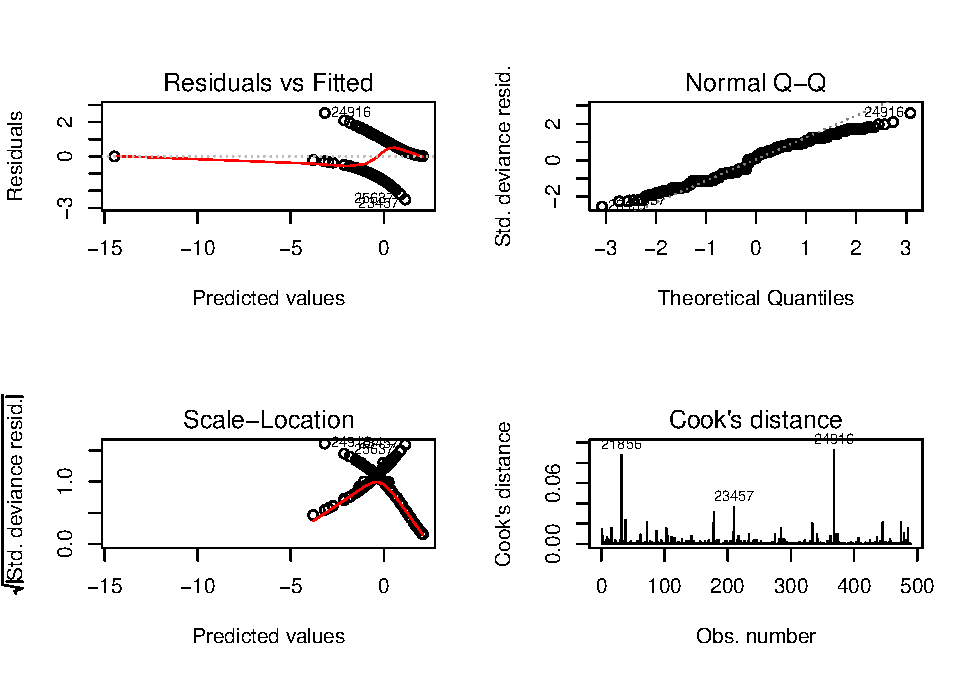
\includegraphics{Dados_Binários1_files/figure-latex/unnamed-chunk-16-1.pdf}

\begin{Shaded}
\begin{Highlighting}[]
\KeywordTok{par}\NormalTok{(}\DataTypeTok{mfrow=}\KeywordTok{c}\NormalTok{(}\DecValTok{2}\NormalTok{,}\DecValTok{2}\NormalTok{))}
\KeywordTok{plot}\NormalTok{(ajuste3, }\DecValTok{1}\OperatorTok{:}\DecValTok{4}\NormalTok{)}
\end{Highlighting}
\end{Shaded}

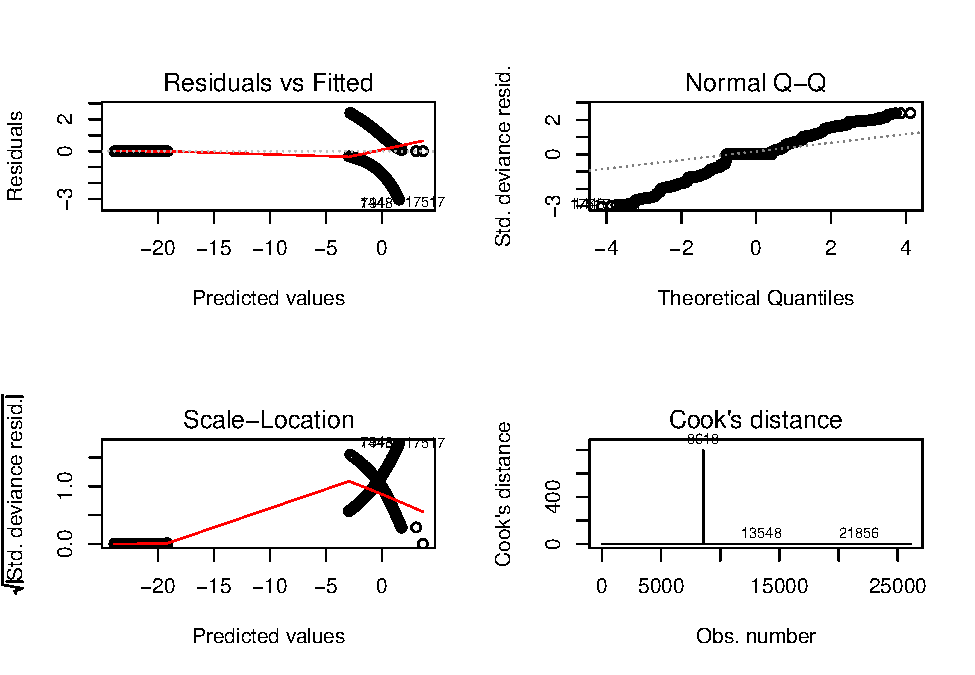
\includegraphics{Dados_Binários1_files/figure-latex/unnamed-chunk-16-2.pdf}

\begin{Shaded}
\begin{Highlighting}[]
\KeywordTok{par}\NormalTok{(}\DataTypeTok{mfrow=}\KeywordTok{c}\NormalTok{(}\DecValTok{1}\NormalTok{,}\DecValTok{2}\NormalTok{))}
\KeywordTok{hnp}\NormalTok{(ajuste3)}
\end{Highlighting}
\end{Shaded}

\begin{verbatim}
## Binomial model
\end{verbatim}

\begin{Shaded}
\begin{Highlighting}[]
\KeywordTok{hnp}\NormalTok{(ajuste3}\FloatTok{.1}\NormalTok{)}
\end{Highlighting}
\end{Shaded}

\begin{verbatim}
## Binomial model
\end{verbatim}

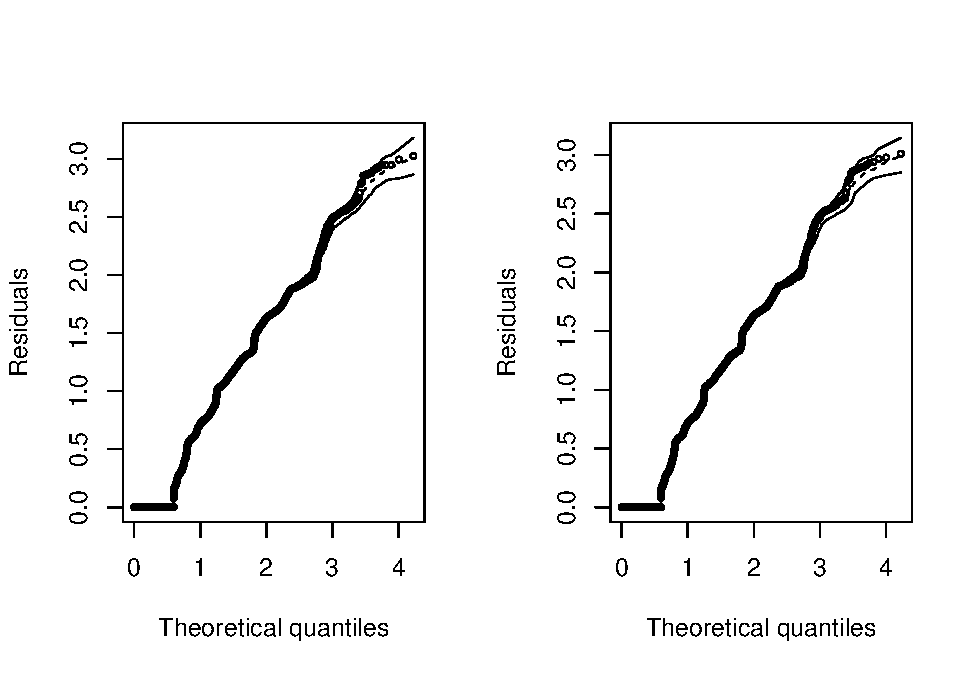
\includegraphics{Dados_Binários1_files/figure-latex/unnamed-chunk-16-3.pdf}

\textbf{5.4 Medidas de Influencia}

\begin{Shaded}
\begin{Highlighting}[]
\KeywordTok{influenceIndexPlot}\NormalTok{(ajuste3}\FloatTok{.1}\NormalTok{, }\DataTypeTok{vars=}\KeywordTok{c}\NormalTok{(}\StringTok{"Cook"}\NormalTok{), }\DataTypeTok{main=}\StringTok{"Distância de Cook"}\NormalTok{)}
\end{Highlighting}
\end{Shaded}

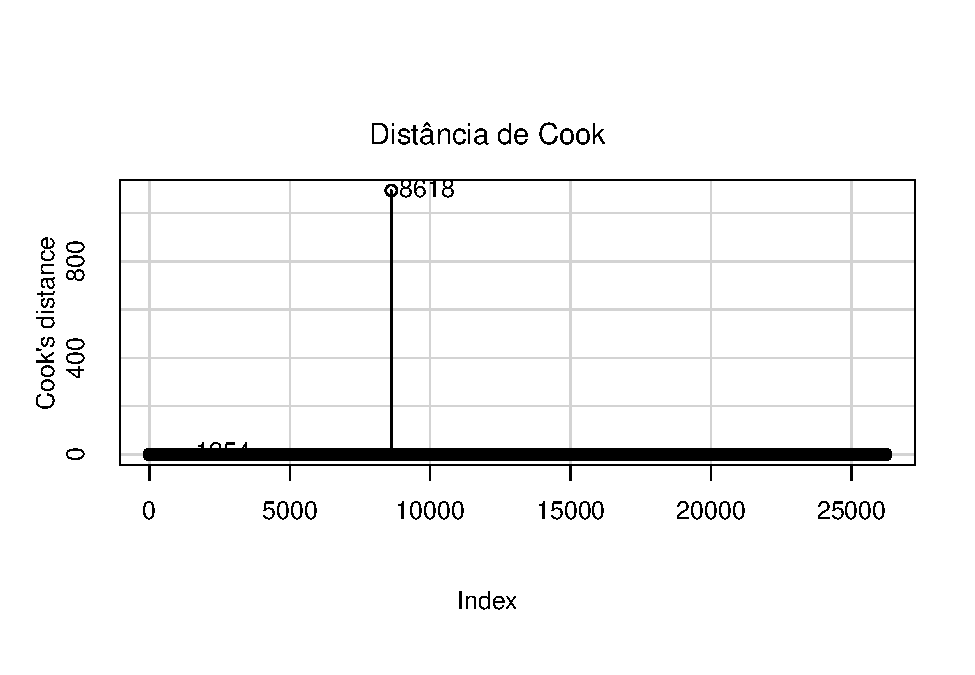
\includegraphics{Dados_Binários1_files/figure-latex/unnamed-chunk-17-1.pdf}

\begin{Shaded}
\begin{Highlighting}[]
\KeywordTok{influenceIndexPlot}\NormalTok{(ajuste3}\FloatTok{.1}\NormalTok{, }\DataTypeTok{vars=}\KeywordTok{c}\NormalTok{(}\StringTok{"Studentized"}\NormalTok{), }\DataTypeTok{main=}\StringTok{"Resíduos Padronizados"}\NormalTok{)}
\end{Highlighting}
\end{Shaded}

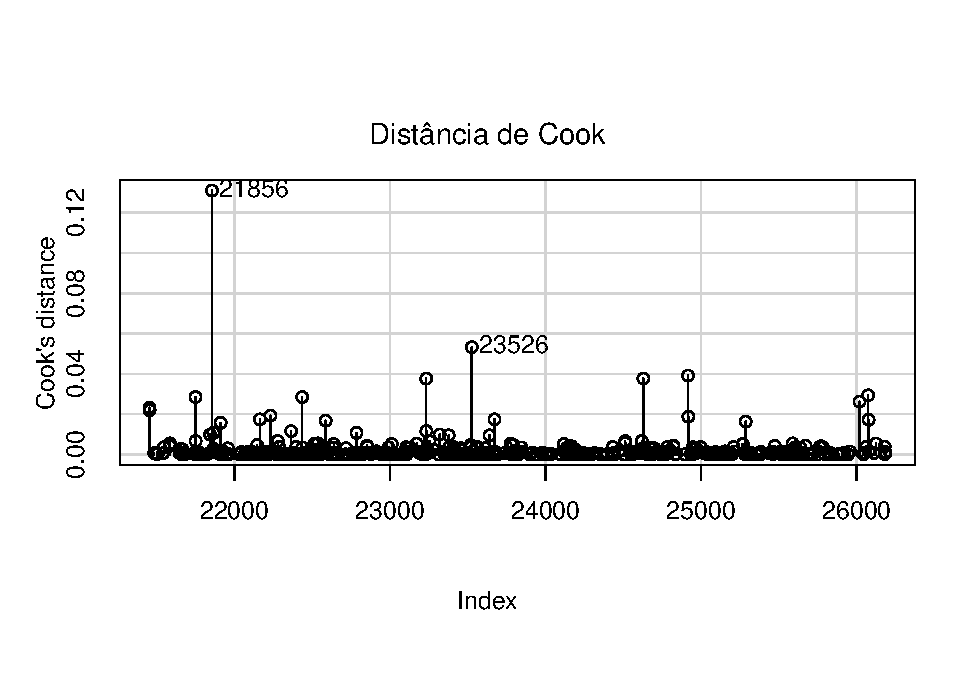
\includegraphics{Dados_Binários1_files/figure-latex/unnamed-chunk-18-1.pdf}

\textbf{5.5 Resíduos Quantílicos Aleatoriazados}

\#\#\textbf{5.6 Gráfico Normal de Probabilidades com Envelope Simulado}
XXXXX Lineu O gráfico de resíduos simulados permite verificar a
adequação do modelo ajustado mesmo que os resíduos não tenham uma
aproximação adequada com a distribuição Normal. Neste tipo de gráfico
espera-se, para um modelo bem ajustado, os pontos (resíduos) dispersos
aleatoriamente entre os limites do envelope.

Deve-se ficar atento à presença de pontos fora dos limites do envelope
ou ainda a pontos dentro dos limites porém apresentando padrões
sistemáticos.

Vamos utilizar a função envelope implementada pelo professor Cesar
Augusto Taconeli :

XXXXX

\begin{Shaded}
\begin{Highlighting}[]
\KeywordTok{par}\NormalTok{(}\DataTypeTok{mfrow=}\KeywordTok{c}\NormalTok{(}\DecValTok{1}\NormalTok{,}\DecValTok{2}\NormalTok{))}
\KeywordTok{hnp}\NormalTok{(ajuste3)}
\end{Highlighting}
\end{Shaded}

\begin{verbatim}
## Binomial model
\end{verbatim}

\begin{Shaded}
\begin{Highlighting}[]
\KeywordTok{hnp}\NormalTok{(ajuste3}\FloatTok{.1}\NormalTok{)}
\end{Highlighting}
\end{Shaded}

\begin{verbatim}
## Binomial model
\end{verbatim}

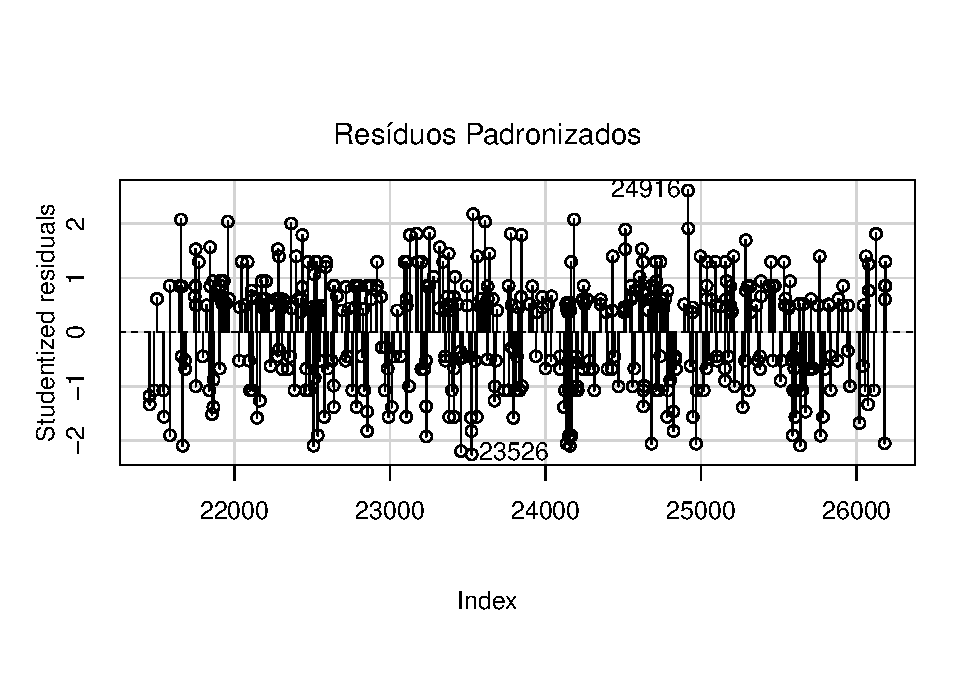
\includegraphics{Dados_Binários1_files/figure-latex/unnamed-chunk-19-1.pdf}

\textbf{5.7 Gráficos de Efeitos}

\begin{Shaded}
\begin{Highlighting}[]
\KeywordTok{plot}\NormalTok{(}\KeywordTok{allEffects}\NormalTok{(ajuste3}\FloatTok{.1}\NormalTok{), }\DataTypeTok{type =} \StringTok{'response'}\NormalTok{, }\DataTypeTok{main =} \StringTok{''}\NormalTok{)}
\end{Highlighting}
\end{Shaded}

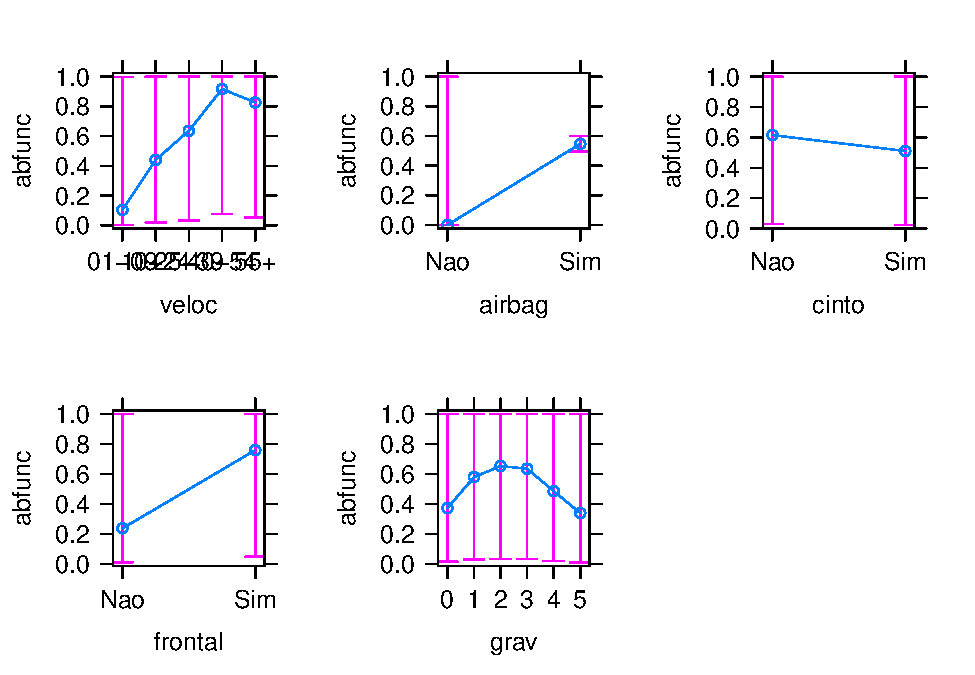
\includegraphics{Dados_Binários1_files/figure-latex/unnamed-chunk-20-1.pdf}

\hypertarget{predicao}{%
\section{6. PREDIÇÃO}\label{predicao}}

\hypertarget{avaliacao-do-poder-preditivo-do-modelo}{%
\section{7. AVALIAÇÃO DO PODER PREDITIVO DO
MODELO}\label{avaliacao-do-poder-preditivo-do-modelo}}

\textbf{7.1 Divisão da Base de dados}

\textbf{7.2 Ponto de Corte}

\textbf{7.3 Sensibilidade e Especificidade}

\textbf{7.4 Curva ROC}

\textbf{7.5 Outra Alternativa de validação}

\hypertarget{referencias}{%
\section{8. REFERÊNCIAS}\label{referencias}}

\hypertarget{section}{%
\section{}\label{section}}


\end{document}
